\chapter{El reloj de Sol -- IV}
\label{sec:el-reloj-de-sol-iv}  

\lettrine[lines=2]{A}{l día siguiente} Cecilia encontró a Antonia en
su oficina ya ubicada frente a la computadora; se sentó a su lado,
decidida a no levantarse sin haber terminado de agujerear todas las
horas de manera óptima y final.

---En el capítulo anterior nos propusimos permitir al lector crear dos
tipos de relojes de Sol: uno con algunas cuantas horas específicas, y
otro presentando todas las que abarquen desde las 6:20 hasta las 17:40
---recordó An\-to\-\mbox{nia---.} Creo que cada uno se merece su propio módulo
---y una vez más arrancó del teclado felices chasquidos.

\section{El reloj de Sol discreto}

\begin{lstlisting}
/* Reloj de Sol de algunas horas puntuales.
  'vector_horas' es un vector con las horas
  y minutos que el usuario desea mostrar;
  por ej.: [[12,00], [7,13], [16,23]]
  representa las 12:00, 7:13 y 16:23.
*/
module reloj_de_sol_discreto(vector_horas){
  difference(){
    cuerpo(largo_reloj);    
    for(hora_minutos=vector_horas){
      hora=hora_minutos[0];
      minutos=hora_minutos[1];
      hora_solar(hora,minutos);    
    }
  }
}
reloj_de_sol_discreto([[12,00],[7,13],[16,23]]);
\end{lstlisting}%

\begin{figure}[ht]
  \centering
  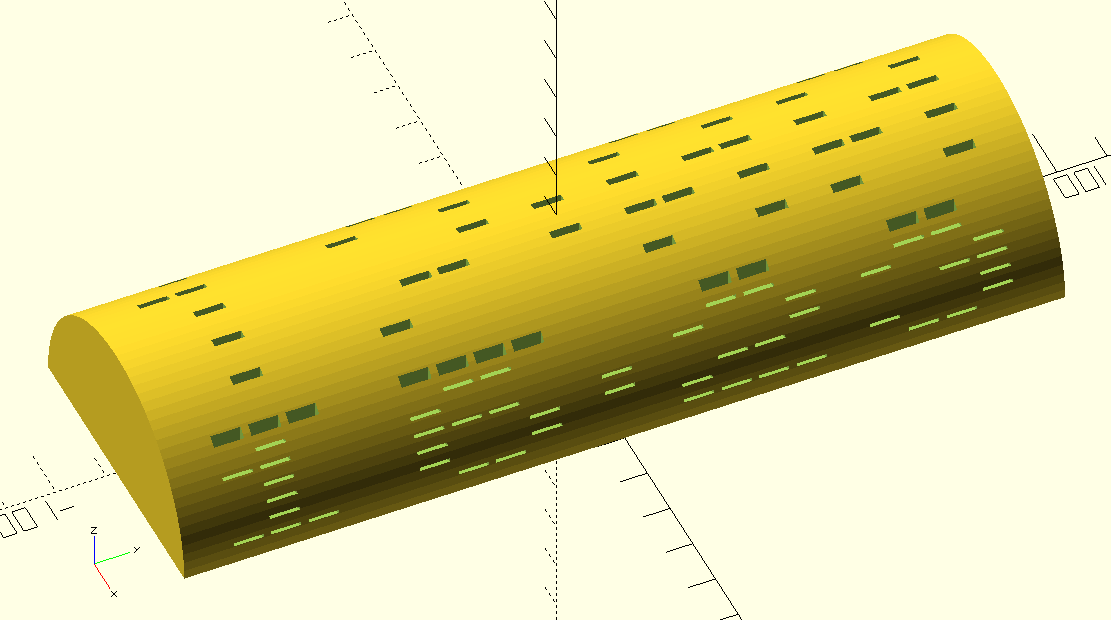
\includegraphics[width=.85\textwidth]{imagenes/reloj-de-sol-discreto}
  \caption{Reloj de Sol discreto, indicando unas cuantas horas
    puntuales.}
  \label{fig:reloj-de-sol-discreto}
\end{figure}

---Cuando un comentario abarca varias líneas es más cómodo encerrarlo
entre las marcas `\lstinline!/*!' y `\lstinline!*/!'  ---aclaró
An\-to\-nia---. Después de todo, creo que este módulo merece un
comentario de alguna extensión: es uno de los dos con los que se
relacionará de manera más directa el lector de este texto.  Los demás
son en cierta manera `auxiliares' ---agregó, como justificándose.

A Cecilia le pareció muy apropiado, y dedicó su atención al módulo: el
bucle de la línea 10 recorría el vector con las horas y minutos que
recibía el módulo como parámetro, almacenando cada pareja en
\lstinline!hora_minutos!. Para cada una, rescataba la \lstinline!hora!
y los \lstinline!minutos! en las líneas 11 y 12, para horadar con ellas
el reloj en la línea 13. No podía ser una solución más sencilla y
elegante.


\section{El reloj de Sol continuo}

---Ahora debemos crear el otro reloj ---Antonia también parecía querer
terminar hoy.


\begin{lstlisting}
module reloj_de_sol_continuo(){
  difference(){
    cuerpo(largo_reloj);    
    // HACER: horas, minutos y separador
  }
}
\end{lstlisting}%

\guillemotright Tanto las decenas como las unidades de las horas y los
minutos, así como el separador, deberán recibir un tratamiento propio
y particular ---volvió a recordar Antonia---.  Empecemos por las
unidades de los minutos, si te parece ---y sin más ceremonia, acercó
el teclado a Cecilia.

\subsection{Las unidades de los minutos}

Cecilia se asombró al descubrir que, a pesar de no saber muy bien lo
que iba a escribir, lo tomaba con seguridad: ya empezaba a comprobar
qué tan cierto era el hecho de que la escritura precedía a la
comprensión de un problema, y no al revés.  Releyó el módulo
\lstinline!hora_solar!; en particular, la sección en la que se
horadaban las unidades de los minutos:

\begin{lstlisting}
// mucho texto antes
   translate([0,8.5*delta_y,0])
      digito(minuto_unidades,alfa,alfa);  
// mucho texto despues
\end{lstlisting}

La variable \lstinline!delta_y! era necesaria para ubicar cada dígito
del reloj; debía incluir su cálculo y definición en el nuevo
módulo. Por lo demás, las unidades de los minutos eran siempre un
redondo cero, abarcando desde las 6:20 a las 17:40:

\begin{lstlisting}
module reloj_de_sol_continuo(){
  delta_y=ancho_pixel+delta_ancho;
  difference(){
    cuerpo(largo_reloj);    
    // unidades de minuto
    translate([0,8.5*delta_y,0])
      digito(0,alfa(6+20/60),alfa(17+40/60));  
    // HACER: el resto
  }
}
reloj_de_sol_continuo();
\end{lstlisting}%

\begin{figure}[ht]
  \centering
  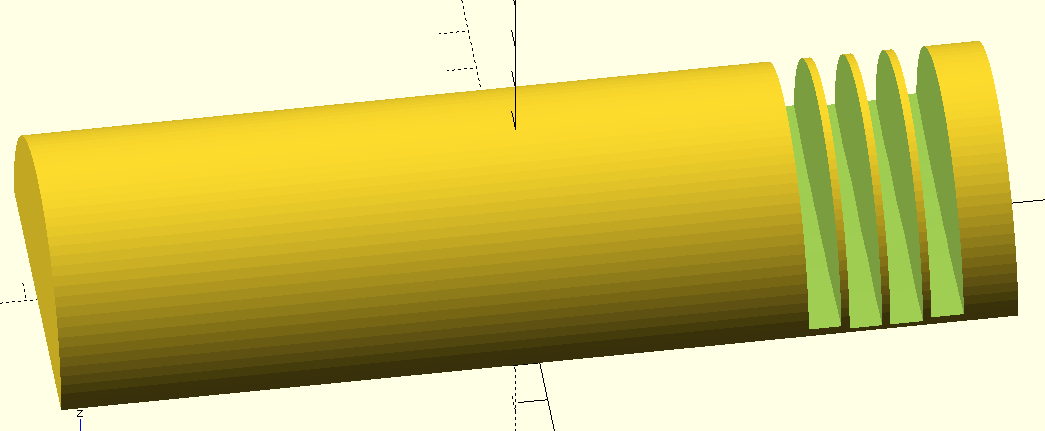
\includegraphics[width=.8\textwidth]{imagenes/unidades-minutos-bug-1}
  \caption{Al intentar agujerear el \texttt{0} de las unidades de los
    minutos, Cecilia tropieza con otro \emph{bug}.}
  \label{fig:unidades-minutos-bug-1}
\end{figure}

\section{Otro \emph{bug} y van...}


Una sonrisa brilló rápidamente en el rostro de Cecilia: el cero
apareció en su lugar, y rebanando limpiamente desde un extremo al otro
el cuerpo del reloj. Sin embargo y con la misma rapidez, su sonrisa se
esfumó. Pudo apreciar un claro problema: ¡El cero parecía no haber
horadado el piso del reloj! Pensó que podía tratarse de un error de la
vista producida por \keystroke{F5}; probó con \keystroke{F6}.

\begin{figure}[ht]
  \centering
  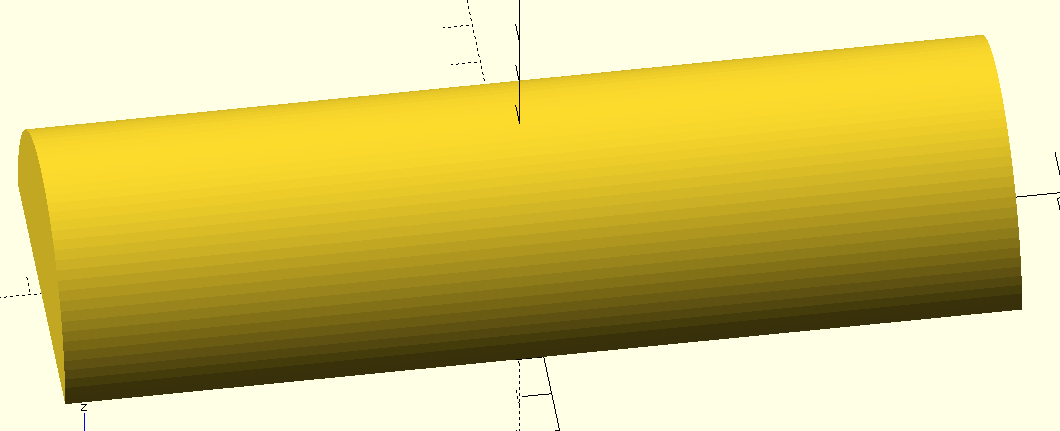
\includegraphics[width=.75\textwidth]{imagenes/unidades-minutos-bug-2}
  \caption{La compilación cabal del reloj no hace desaparecer el
    problema; antes bien, lo manifiesta con mayor crudeza.}
  \label{fig:unidades-minutos-bug-2}
\end{figure}

¡Horror! ¡La figura \ref{fig:unidades-minutos-bug-2} acusaba que ahora
las mismas rebanadas desaparecían!  Giró hacia Antonia en busca de
ayuda; no le sorprendió demasiado encontrarla sonriendo.

---A mí me pasó exactamente lo mismo ---confesó su a\-mi\-ga---. Es un
\emph{bug} bastante sutil; fijate ---adelantó, tomando el teclado:

\begin{lstlisting}
echo(alfa(6+20/60));
echo(alfa(17+40/60));
\end{lstlisting}


\begin{figure}[ht]
  \centering
  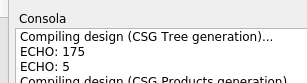
\includegraphics[width=.6\textwidth]{imagenes/unidades-minutos-bug-3}
  \caption{Antonia señala el origen profundo del \emph{bug}.}
  \label{fig:unidades-minutos-bug-3}
\end{figure}


Cecilia miró el resultado de la consola en la figura
\ref{fig:unidades-minutos-bug-3} sin comprender nada aún.

---A las 6:20 le corresponde un ángulo $\alpha$ más grande que a las
17:40 ---señaló Antonia.

Cecilia podía verlo con toda claridad:

---¿Y? ---preguntó, sin disimular una nota de mal humor.

Antonia, ahora sin decir palabra, escribió un ejemplo más:

\begin{lstlisting}[numbers=none]
digito(0,alfa(12),alfa(13));
\end{lstlisting}


\begin{figure}[ht]
  \centering
  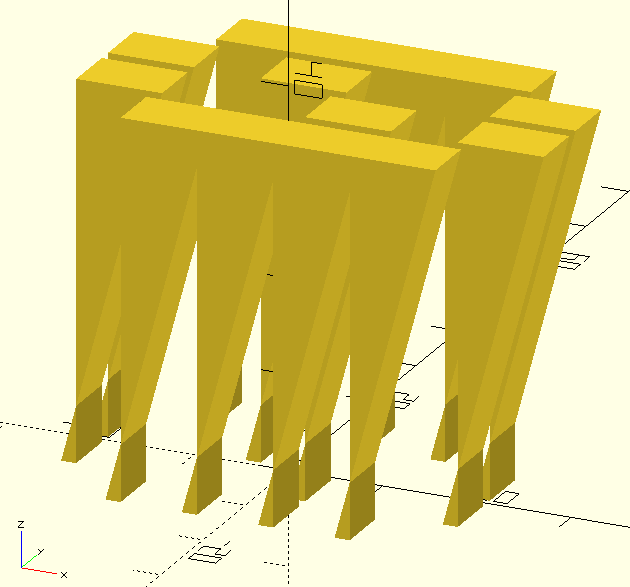
\includegraphics[width=.51\textwidth]{imagenes/unidades-minutos-bug-4}
  \caption{Antonia exhibe el resultado de pretender construir un rayo
    de Sol en el que $\alpha_1>\alpha_2$.}
  \label{fig:unidades-minutos-bug-4}
\end{figure}


Cecilia pareció querer lanzarse sobre la figura
\ref{fig:unidades-minutos-bug-4}: ahora le parecía empezar a
comprender el problema. Si el ángulo inicial del haz de rayos era
mayor al ángulo final ($\alpha_1>\alpha_2$), la geometría conquistada
en el capítulo \ref{sec:el-reloj-de-sol-iii} se trastocaba, haciendo
que los extremos superiores del haz resultaran ``intercambiados''
entre sí, con lo que el polígono presentaba una rara intersección
interna.

\begin{figure}[ht]
  \centering
  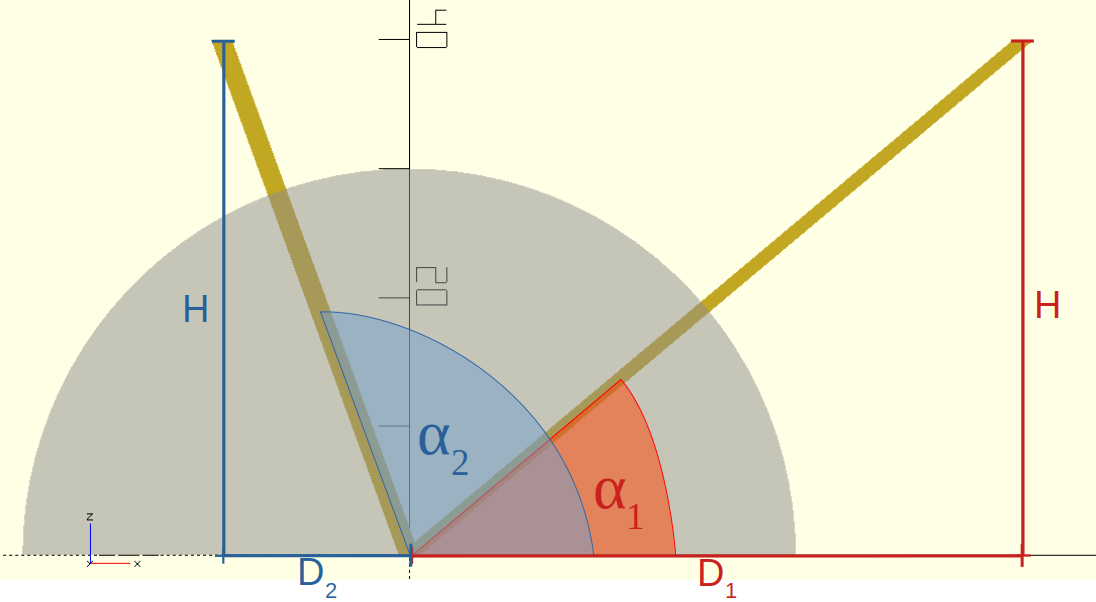
\includegraphics[width=.6\textwidth]{imagenes/dos-rayos-anotados}
  \caption{El algoritmo que Antonia y Cecilia discurrieron en el
    capítulo \ref{sec:el-reloj-de-sol-iii} para crear un haz de rayos
    suponía que $\alpha_1 < \alpha_2$; en caso contrario, $D_1$ y $D_2$
    se trastocan y el polígono resultante no puede ser extrudido
    válidamente.}
  \label{fig:alfas-cap-28}
\end{figure}

---Un polígono así construido, una vez extrudido, no es un objeto
tridimensional legítimo ---explicó Antonia---.  \openscad{} no puede
determinar cuál es su interior y cuál su exterior. De hecho, si vos
hacés \keystroke{F6} se va a quejar, como podés comprobar en la figura
\ref{fig:unidades-minutos-bug-5}.


\begin{figure}[ht]
  \centering
  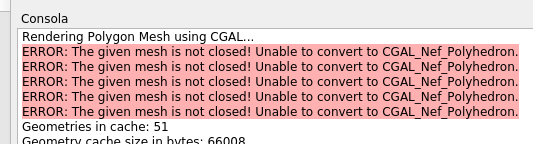
\includegraphics[width=.99\textwidth]{imagenes/unidades-minutos-bug-5}
  \caption{La consola acusa la invalidez del haz de rayos contruido
    con $\alpha_1>\alpha_2$.}
  \label{fig:unidades-minutos-bug-5}
\end{figure}

---¡Pues bien! Entonces la solución es fácil ---dijo Cecilia,
recuperando el teclado con entusiasmo.

\begin{lstlisting}
module reloj_de_sol_continuo(){
  delta_y=ancho_pixel+delta_ancho;
  difference(){
    cuerpo(largo_reloj);    
    // unidades de minuto
    translate([0,8.5*delta_y,0])
      digito(0,alfa(17+40/60),alfa(6+20/60));
    // HACER: el resto
  }
}
reloj_de_sol_continuo();
\end{lstlisting}%

\begin{figure}[ht]
  \centering
  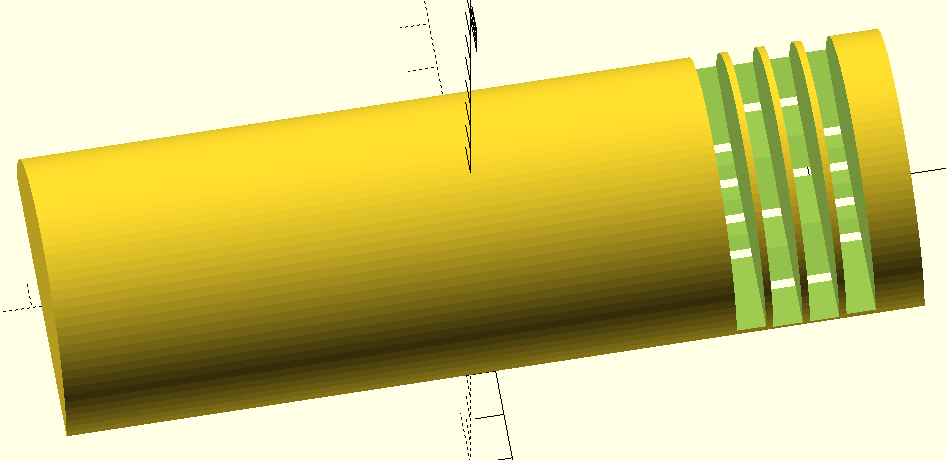
\includegraphics[width=.75\textwidth]{imagenes/unidades-minutos}  
  \caption{Cecilia soluciona el \emph{bug}... aparentemente.}
  \label{fig:unidades-minutos}
\end{figure}

Antonia, aun ante la figura \ref{fig:unidades-minutos}, no parecía
satisfecha:

---El problema es que ahora va a funcionar para lectores del
hemisferio sur; para los boreales, a las 17:40 les corresponde un
ángulo mayor que a las 6:20 ---dijo, recuperando el teclado.

\begin{lstlisting}
hemisferio="norte";
echo(alfa(6+20/60));
echo(alfa(17+40/60));
\end{lstlisting}%

\begin{figure}[ht]
  \centering
  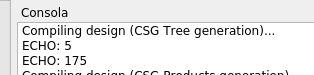
\includegraphics[width=.6\textwidth]{imagenes/unidades-minutos-bug-6}
  \caption{Antonia demuestra que la solución rápidamente ofrecida por
    Cecilia no es tal.}
  \label{fig:unidades-minutos-bug-6}
\end{figure}


Cecilia se derrumbó contra el respaldo de la silla; volvió a sentir
que el reloj de Sol se alejaba una vez más. ¿Podrían terminarlo hoy?
¿Podrían terminarlo alguna vez? Se sentía al borde del desánimo, pero
se obligó a pensar una solución; tras unos instantes, aventuró:

---¿Lo arreglamos con un \lstinline!if!?

---Podría ser, pero antes debemos decidir dónde lo hacemos ---aconsejó
Antonia---. En este módulo me parece mala idea: no es su
responsabilidad traficar con ángulos, sino con horas: ¿qué pueden
importarle esos detalles de implementación? Además, imaginate que en
un futuro, releyendo el texto, decidimos que es mejor medir los
ángulos desde el mediodía en lugar de hacerlo desde el horizonte:
tendríamos que modificar este módulo también.

A Cecilia ya le estaba costando imaginarse terminando el reloj; no
hablemos ya de releerlo en un futuro. Pero eligió seguir acompañando a
su amiga.

---\lstinline!reloj_de_sol_continuo! invoca al módulo
\lstinline!digito!, el cual sólo recibe los ángulos extremos para
pasarlos a \lstinline!haz_de_sol! ---re\-ca\-pi\-tu\-ló Antonia---.  Es este
último módulo el que debe asegurarse de que $\alpha_1$ sea menor que
$\alpha_2$ ---aseguró.

\section{Funciones \texttt{min} y \texttt{max}}

---Podríamos usar un \lstinline!if!, o incluso el operador ternario
`\lstinline!? :!' ---concedió Antonia---. Pero creo que es más piola
aprovechar las funciones \lstinline!min! y \lstinline!max!: la primera
te devuelve el menor de los valores que le pasás como argumentos, y la
segunda... bueno, ya lo habrás imaginado:

\begin{lstlisting}
echo(min(5,1,2,10,3));
echo(max(5,1,2,10,3));
\end{lstlisting}%

\begin{figure}[ht]
  \centering
  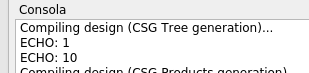
\includegraphics[width=.6\textwidth]{imagenes/min-max}  
  \caption{Antonia muestra el empleo de las funciones \lstinline!min!
    y \lstinline!max!.}
  \label{fig:min-max}
\end{figure}

\guillemotright Con esas funciones, la modificación es relativamente
trivial: ---afirmó Antonia.

\begin{lstlisting}
module haz_de_sol(alfa1,alfa2){
  alfa_min=min(alfa1,alfa2);
  alfa_max=max(alfa1,alfa2);
  D1=H/tan(alfa_min);
  D2=H/tan(alfa_max);
  vertices=[[-alto_pixel/2,0],
            [D2-alto_pixel/2,H],
            [D1+alto_pixel/2,H],
            [alto_pixel/2,0]];
  // TODO: medir la duracion de esta solucion
  //       y la de esta otra:
  //       translate([0,ancho_pixel/2,0])
  //       Ojo : borrar 'center=true' abajo
  rotate([90,0,0])
    linear_extrude(ancho_pixel,center=true)
      polygon(vertices);
}\end{lstlisting}%
% \begin{center}
% % \begin{minipage}[b]{.25\textwidth}\vspace{0pt}
% %     \centering
%   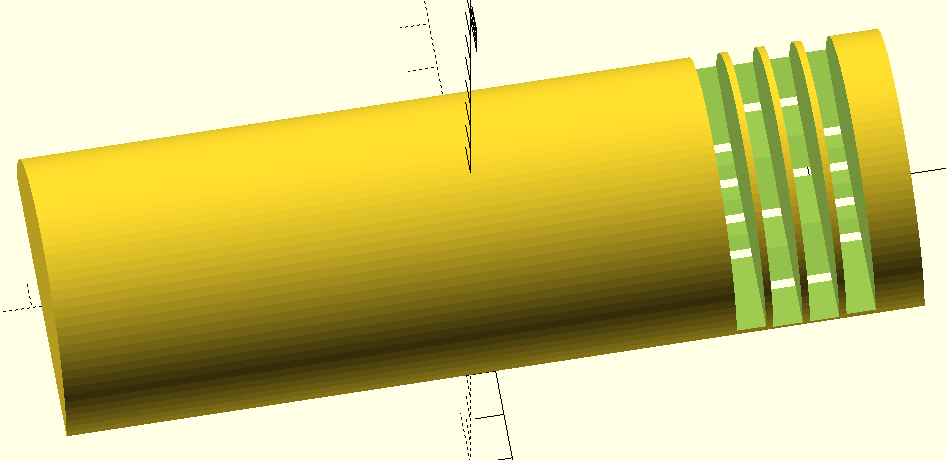
\includegraphics[width=.4\textwidth]{imagenes/unidades-minutos}
% % \end{minipage}
% \end{center}

A Cecilia le gustó la solución: en las líneas 2 y 3 se obtenían el
menor y el mayor de los valores de $\alpha_1$ y $\alpha_2$, y con
ellos se calculaban $D_1$ y $D_2$ en las líneas 4 y 5. Además,
cualquier modificación futura referente al tratamiento de los ángulos
quedaba encapsulada en este módulo, por lo que no debería ser muy
difícil de llevar a cabo. Pero lo mejor de todo es que... ¡Funcionaba!

\begin{lstlisting}
hemisferio="sur";
reloj_de_sol_continuo();
\end{lstlisting}%

\begin{figure}[ht]
  \centering
  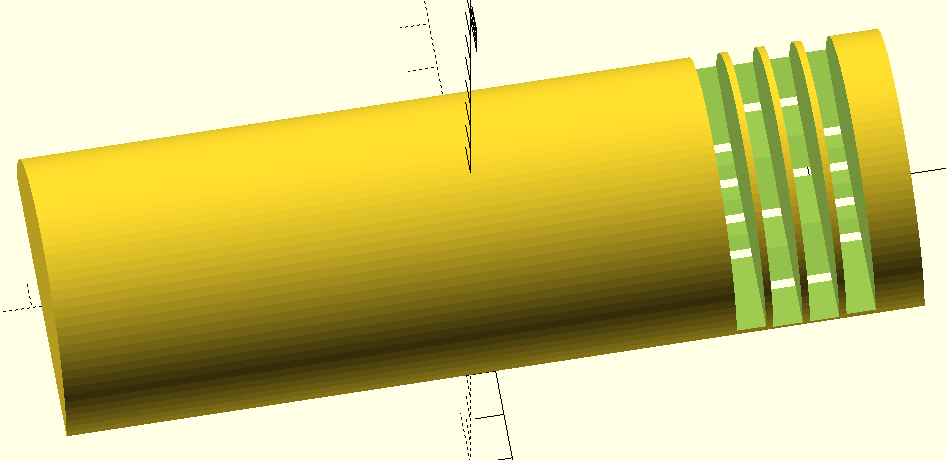
\includegraphics[width=.85\textwidth]{imagenes/unidades-minutos}
  \caption{La solución de Antonia funciona para el hemisferio sur...}
  \label{fig:unidades-sur}
\end{figure}

\begin{lstlisting}
hemisferio="norte";
reloj_de_sol_continuo();
\end{lstlisting}%

\begin{figure}[ht]
  \centering
  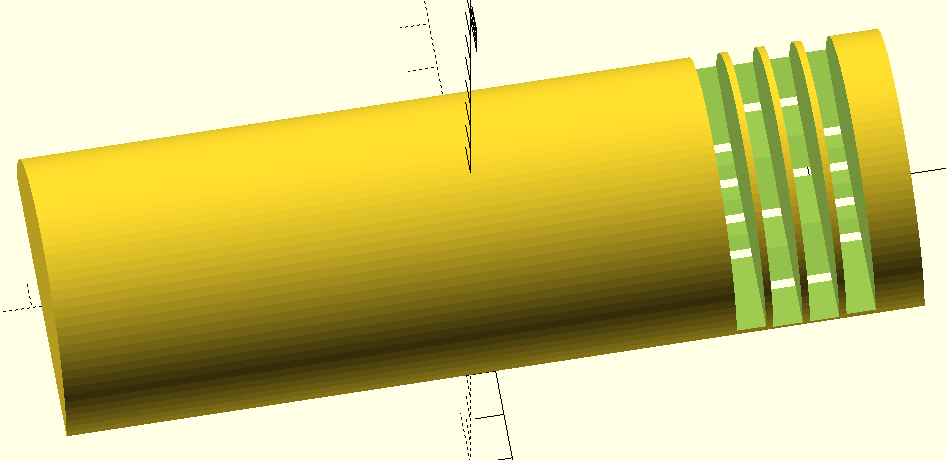
\includegraphics[width=.85\textwidth]{imagenes/unidades-minutos}  
  \caption{...y para el hemisferio norte.}
  \label{fig:unidades-norte}
\end{figure}

\subsection{Las decenas de los minutos}

---Ahora es el turno de las decenas de los minutos ---dijo Antonia
cediendo nuevamente el teclado a Cecilia, quien lo tomó mientras
releía el módulo \lstinline!hora_solar! para inspirarse.

\begin{lstlisting}
 // [...]
 minuto_decenas=n_a_digito(minutos,1);
 // [...]
  translate([0,3.5*delta_y,0])
    digito(minuto_decenas,alfa,alfa);
 // [...]
\end{lstlisting}

Al menos superficialmente las decenas resultaban muy parecidas a las
unidades; la mayor diferencia parecía ser que el dígito no era siempre
el mismo, sino que debía fluctuar entre 0, 2 y 4. Aunque examinándolo
con mayor atención descubrió que el problema era más arduo de lo que
parecía: ¡Los ángulos $\alpha_1$ y $\alpha_2$ dependían no sólo de los
minutos, sino de la hora completa!

Tras unos instantes en los que se sintió prácticamente paralizada,
decidió que simplemente mirando y pensando no iba a llegar a ningún
lado; por lo que se lanzó a escribir, confiando en sus siempre fieles
\keystroke{Supr} y \keystroke{$\Longleftarrow$}. Al cabo de unos
intensos minutos, que para ella transcurrieron en un espacio fuera del
tiempo, logró lo siguiente:

\begin{lstlisting}
module reloj_de_sol_continuo(){
  delta_y=ancho_pixel+delta_ancho;
  difference(){
    cuerpo(largo_reloj);    
    // unidades de minuto
    translate([0,8.5*delta_y,0])
      digito(0,alfa(6+20/60),alfa(17+40/60));  
    // decenas de minuto
    translate([0,3.5*delta_y,0])
      for(hora=[6:17],
          minutos=[0,20,40])
        if((hora+minutos/60) > 6) {
          minuto_decenas=n_a_digito(minutos,1);
          digito(minuto_decenas,
                 alfa(hora+minutos/60),
                 alfa(hora+minutos/60));
          }
  }
}
reloj_de_sol_continuo();
\end{lstlisting}


\begin{figure}[ht]
  \centering
  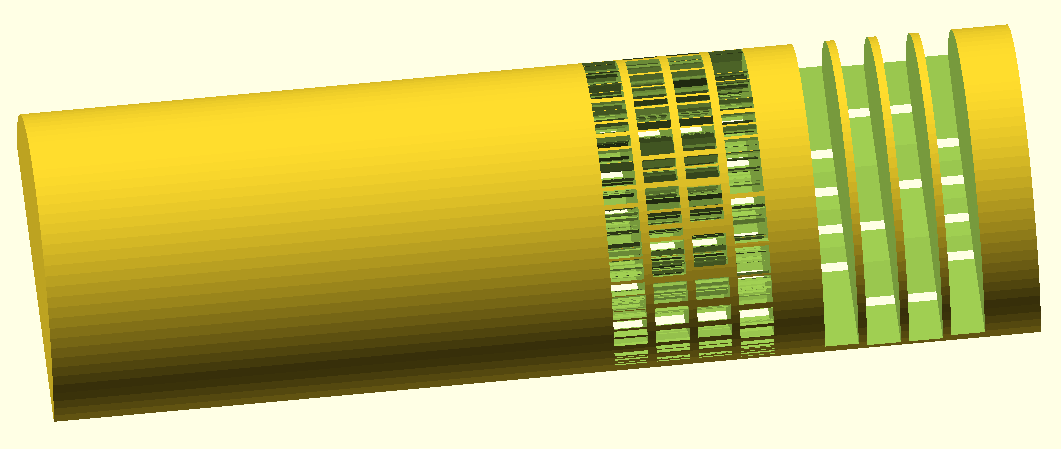
\includegraphics[width=.85\textwidth]{imagenes/decenas-minutos-1}  
  \caption{Cecilia logra horadar el reloj con las decenas de los
    minutos.}
  \label{fig:decenas-minutos-1}
\end{figure}


Una vez escrito no le pareció tan difícil... ¡Pero le costó lo suyo!
Y por eso mismo estaba más contenta releyendo su nuevo texto y
contemplando el resultado en la figura \ref{fig:decenas-minutos-1}.

La línea 9 se encargaba de ubicar el dígito en su lugar. En las líneas
10 y 11 se declaraba el doble bucle que asignaba a \lstinline!hora!
los valores del 6 al 17 y a \lstinline!minutos! las valores 0, 20 y
40: de esta manera se recorrían todas las horas desde las 6:00 a las
17:40 en intervalos de 20 minutos. Para evitar las conflictivas 6:00,
decidió anteponer a la creación del dígito un \lstinline!if! en la
línea 12.

En la línea 13 se rescataba el dígito a horadar, y finalmente las
líneas 14 a 16 se encargaban del trabajo tan delicadamente preparado
por las anteriores.

Antonia sólo sonreía, feliz.

\subsection{El separador}

El separador le recordó las unidades de los minutos: un único símbolo
abarcando las horas extremas.

\begin{lstlisting}
module reloj_de_sol_continuo(){
  delta_y=ancho_pixel+delta_ancho;
  difference(){
    cuerpo(largo_reloj);    
    // unidades de minuto
    translate([0,8.5*delta_y,0])
      digito(0,alfa(6+20/60),alfa(17+40/60));  
    // decenas de minuto
    translate([0,3.5*delta_y,0])
      for(hora=[6:17],
          minutos=[0,20,40])
        if ((hora+minutos/60)>6) {
          minuto_decenas=n_a_digito(minutos,1);
          digito(minuto_decenas,
                 alfa(hora+minutos/60),
                 alfa(hora+minutos/60));
          }
    // separador
    separador(alfa(6+20/60),alfa(17+40/60));  
  }  
}
reloj_de_sol_continuo();
\end{lstlisting}%


\begin{figure}[ht]
  \centering
  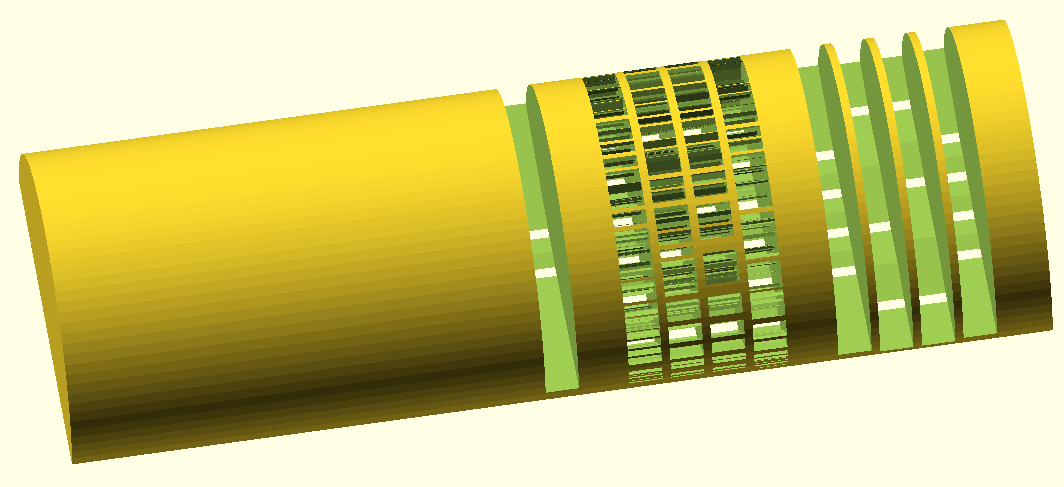
\includegraphics[width=.85\textwidth]{imagenes/separador-continuo}  
  \caption{Cecilia agrega el separador de horas y minutos.}
  \label{fig:separador-continuo}
\end{figure}


Cecilia giró para mirar a Antonia. Tal vez por primera vez desde que
comenzaron esta aventura, ninguna de las dos supo qué decir.

\subsection{Las unidades de la hora}

Sólo faltaban dos dígitos; Cecilia sentía que ya nada las podía
detener. Con entusiasmo y una confianza dichosa se lanzó a escribir
casi sin detenerse antes a pensar. Si la pulsación de las teclas
\keystroke{Supr} y \keystroke{$\Longleftarrow$} ocuparan sitio en el
texto, este manual doblaría la cantidad de sus páginas; afortunadamente
no es así.

\begin{lstlisting}
module reloj_de_sol_continuo(){
  delta_y=ancho_pixel+delta_ancho;
  difference(){
    cuerpo(largo_reloj);    
    // unidades de minuto
    translate([0,8.5*delta_y,0])
      digito(0,alfa(6+20/60),alfa(17+40/60));  
    // decenas de minuto
    translate([0,3.5*delta_y,0])
      for(hora=[6:17],
          minutos=[0,20,40])
        if ((hora+minutos/60)>6) {
          minuto_decenas=n_a_digito(minutos,1);
          digito(minuto_decenas,
                 alfa(hora+minutos/60),
                 alfa(hora+minutos/60));
          }
    // separador
    separador(alfa(6+20/60),alfa(17+40/60));  
    // unidades de hora
    translate([0,-3.5*delta_y,0])
      for(hora=[6:17]){
        hora_unidades=n_a_digito(hora,0);
        digito(hora_unidades,
               alfa(hora>6?hora:hora+20/60),
               alfa(hora>6?hora:hora+20/60));
      }
  }  
}
reloj_de_sol_continuo();
\end{lstlisting}%


\begin{figure}[ht]
  \centering
  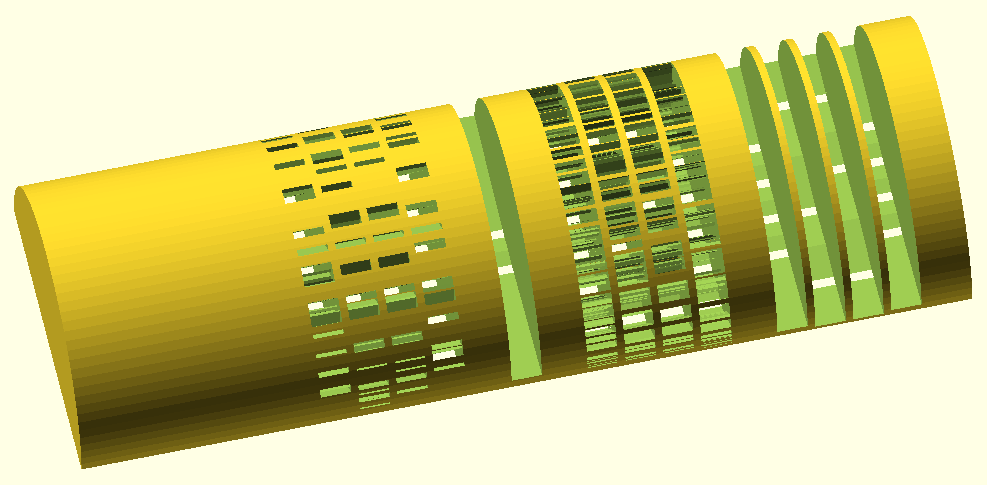
\includegraphics[width=.85\textwidth]{imagenes/hora-unidades-1}  
  \caption{Cecilia añade al reloj las unidades de las horas.}
  \label{fig:hora-unidades-1}
\end{figure}

Cecilia saludó con una amplia sonrisa el resultado desplegado en la
figura \ref{fig:hora-unidades-1}, mientras volvía a satisfacer su
vanidad releyendo su flamante texto. Ahora sólo era necesario recorrer
las horas mediante un bucle en la línea 22. En la 23 obtenía sus
unidades. Por último, sólo restaba agujerear el reloj con el dígito
correspondiente en las líneas 24 a 26.

Estaba particularmente orgullosa por la forma en que había evitado las
siempre conflictivas 6:00: mediante el operador ternario
`\lstinline!? :!' indagaba si \lstinline!hora! era mayor a 6. En caso
afirmativo, $\alpha$ se calculaba simplemente usando la hora; en caso
contrario, se le sumaban 20 minutos a la misma, calculando así
efectivamente el ángulo para las 6:20. Se sentía muy astuta.

Cuando quiso compartir su dicha con Antonia, la encontró con un gesto
ambiguo. Automáticamente se puso en guardia: se preparó para el
implacable baldazo de agua fría. Sin embargo, se sorprendió al
descubrir que esa actitud instintiva no era acompañada de una
sensación de abatimiento: de alguna manera había logrado confiar en
que podría resolver los problemas que se interpusieran entre ella y el
reloj de Sol digital. Este pensamiento la hizo más feliz, quizá, que
el hecho de conseguirlo en sí mismo.

---¿Qué hay ahora, Antonia? ¿Qué debemos solucionar?  ---pre\-gun\-tó
Cecilia, con una sonrisa confiada.

Antonia pareció adivinar sus sensaciones, porque le devolvió una
sonrisa en la que brillaba una luz que podría decirse de orgullo ante
la saludable evolución operada en Cecilia, que ---co\-mo casi cualquier
docente--- creía ingenuamente poder atribuir a su eficacia didáctica:

---Acabás de agujerear el reloj con horas \emph{justas}. Tal vez
\emph{demasiado} justas ---observó, enigmática---. Las 12:00 te quedan
perfectas, pero... ¿Qué observaremos a las, digamos, 12:20?

\begin{lstlisting}
$vpr=[90-alfa(12),0,90];
reloj_de_sol_continuo();
\end{lstlisting}%$


\begin{figure}[ht]
  \centering
  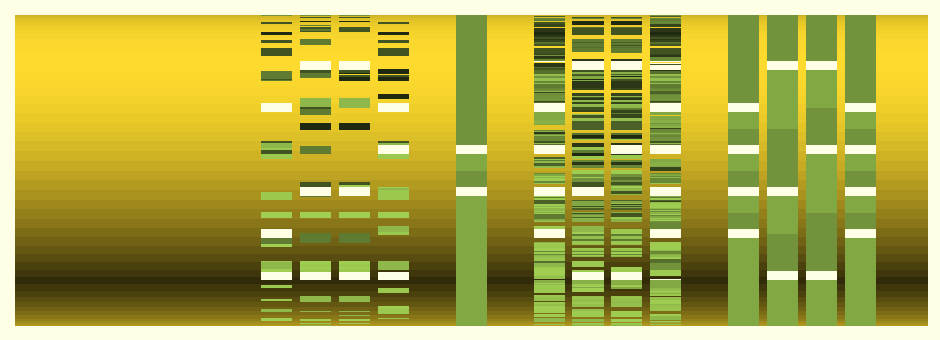
\includegraphics[width=.8\textwidth]{imagenes/hora-unidades-3}
  \caption{Antonia muestra que las 12:00 se observan perfectamente...}
  \label{fig:hora-unidades-3}
\end{figure}


\begin{lstlisting}
$vpr=[90-alfa(12+20/60),0,90];
reloj_de_sol_continuo();
\end{lstlisting}%$


\begin{figure}[ht]
  \centering
  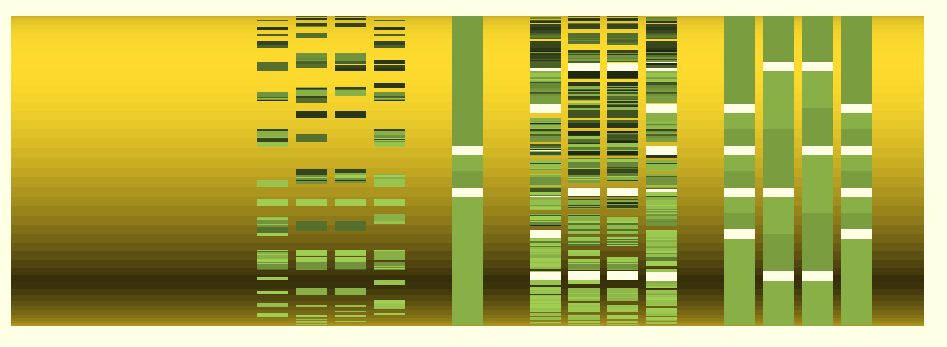
\includegraphics[width=.8\textwidth]{imagenes/hora-unidades-2}
  \caption{...pero las que 12:20 no, debido a que Cecilia horadó las
    horas con \emph{demasiada} justeza.}
  \label{fig:hora-unidades-2}
\end{figure}


---¡Es verdad! ---exclamó Cecilia, con sorpresa pero sin temor frente
a las correspondientes figuras \ref{fig:hora-unidades-3} y
\mbox{\ref{fig:hora-unidades-2}---.} Los haces son demasiado estrechos: deben
abarcar una hora, después de todo ---y con entusiasmo se dispuso a
enmendar el texto.

\begin{lstlisting}
// [...]
// unidades de hora
translate([0,-3.5*delta_y,0])
  for(hora=[6:17]){
    hora_unidades=n_a_digito(hora,0);
    digito(hora_unidades,
           alfa(hora>6?hora:hora+20/60),
           alfa(hora+59/60));
  }
// [...]
$vpr=[90-alfa(12+20/60),0,90];
reloj_de_sol_continuo();
\end{lstlisting}%$


\begin{figure}[ht]
  \centering
  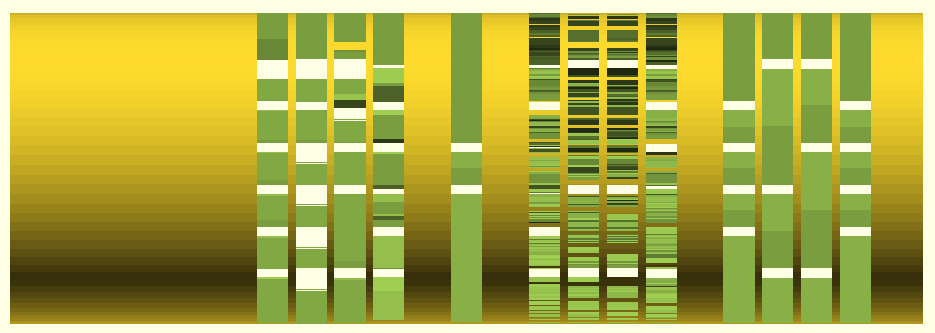
\includegraphics[width=.9\textwidth]{imagenes/hora-unidades-5}  
  \caption{Cecilia extiende al haz de las horas 59 minutos...}
  \label{fig:hora-unidades-5}
\end{figure}


El resultado exhibido en la figura \ref{fig:hora-unidades-5} no era
francamente el que Cecilia esperaba, y eso que sólo había modificado
la línea 8, extendiendo el haz de cada hora hasta el minuto 59. Rotó
un poco el reloj para ver si obtenía una pista de lo que estaba
ocurriendo.


\begin{figure}[ht]
  \centering
  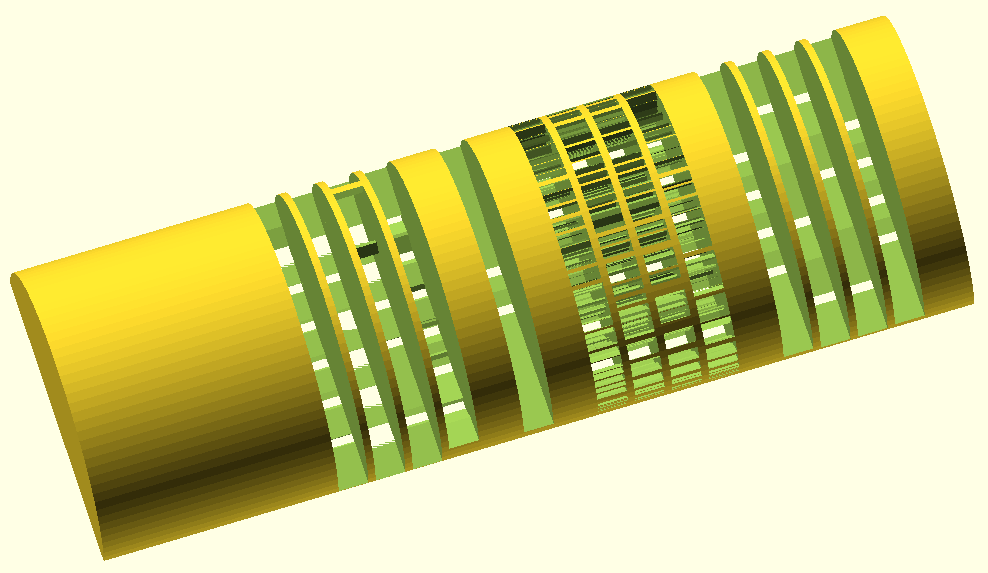
\includegraphics[width=.95\textwidth]{imagenes/hora-unidades-4}  
  \caption{...pero eso, ahora, parece excesivo.}
  \label{fig:hora-unidades-4}
\end{figure}


---¡Claro! ---dijo, mientras reía y se cubría los ojos con una mano,
tras enfrentarse al resultado expuesto en la figura
\ref{fig:hora-unidades-4}---. ¡Ahora el haz es demasiado extenso! En
esencia recaí en el error que habíamos cometido en el capítulo
\ref{sec:el-reloj-de-sol-i} al trazar \emph{todas} las horas y los
minutos: rebanamos el cuerpo entero del reloj.

---Exacto ---confirmó Antonia---. Hay que usar un haz más amplio, pero
no tanto como para que una hora se solape con la siguiente.

Cecilia expresó su acuerdo con un lento movimiento de cabeza:

---¿Y qué tan amplio debe ser? ---indagó.

Antonia suspiró con fuerza, mientras se recostaba contra el respaldo
de la silla:

---Te confieso que ésta es la parte que más me costó definir en la
versión del reloj que escribí hace tiempo... Lo mejor es ir probando
---sugirió.

Cecilia lo hizo con varios valores en la línea 8, pero ninguno parecía
funcionar: o la hora en cuestión se ``apagaba'' antes de tiempo ---si
el haz era demasiado estrecho--- o se mezclaba con una contigua ---si
era demasiado amplio.

Cuando estaba empezando a cansarse de probar, Antonia por fin se
decidió a intervenir:

---Esas horas son un problema, ciertamente ---con\-fir\-\mbox{mó---.} Cuando
llegué a este punto me decidí a mirar el texto del creador del reloj
original.\footnote{No está de más recordar aquí el origen de la
  inspiración del reloj:
  \url{https://www.thingiverse.com/thing:1068443}. (Nota del Editor)}
Tomó un par de decisiones que llamaron mi atención: la altura de cada
pixel era de apenas $0.75$ mm, y las horas agujereadas iban desde las
10:00 a las 16:00.

Cecilia abrió los ojos con asombro:

---¿Tan pocas horas?  ---preguntó.

---Sí ---respondió Antonia, encogiéndose de hombros---.  Tal vez es la
única manera que encontró de resolver esta cuestión.

Cecilia decidió darle una oportunidad al tamaño del pixel, pero le
parecía una pena renunciar a tantas horas del día. Sin embargo, y
después de mucho probar, lo mejor que consiguió fue desplazar una hora
el mismo conjunto de 6 horas, abarcando así un intervalo más simétrico
desde las 9:00 a las 15:00:

\begin{lstlisting}
alto_pixel = .75; // Era 1.6 y antes 2
// [...]
// unidades de hora
translate([0,-3.5*delta_y,0])
  for(hora=[9:15]){
        hora_unidades=n_a_digito(hora,0);
        digito(hora_unidades,
               alfa(hora),
               alfa(hora<15 ? hora+50/60: hora+10/60));
      }
// [...]
$vpr=[90-alfa(12+40/60),0,90];
reloj_de_sol_continuo();
\end{lstlisting}%$


\begin{figure}[ht]
  \centering
  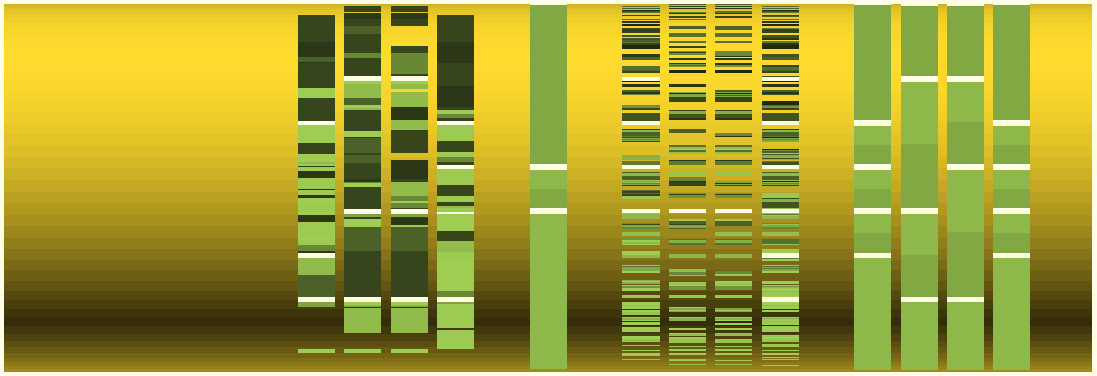
\includegraphics[width=.95\textwidth]{imagenes/hora-unidades-6}  
  \caption{Cecilia se resigna a horadar el reloj con las horas
    comprendidas entre las 9:00 y las 15:00. Además, usa pixeles menos
    altos.}
  \label{fig:hora-unidades-6}
\end{figure}


En la línea 5 el bucle se resignaba a las horas que iban desde las 9 a
las 15. Cada una de ellas se extendía durante 50 minutos en la línea 9
(salvo las 15:00, que se prolongaban sólo 10 minutos), por lo que el
``día'' del reloj acababa reduciéndose al intervalo que iba desde las
9:00 a las 15:10.

Cecilia sentía una mezcla agridulce de sensaciones, en las que se
entrelazaban la nostalgia por haber perdido la totalidad de las horas
diurnas y la alegría de estar a un dígito de terminar su ansiado
reloj. Mientras releía su texto reconoció que en última instancia
primaba una suerte de dicha: reconoció en esa mezcla indecisa y
anhelante un efecto muy parecido al que le producían la música, la
literatura y el arte en general; esa inquietante impresión que
describió Edgar Allan Poe con una admirable queja: el Arte nos depara
la felicidad y la congoja de quien ve los Cielos súbitamente abiertos
para inmediatamente después encontrarlos cerrados y ocultos tras un
denso y opaco velo.

Antonia la devolvió bruscamente a la realidad:

---¿Qué hacemos ahora con los minutos? ---preguntó.

Cecilia emergió de sus pensamientos con cierta alarma:

---¿Cómo qué hacemos? Ya está; ya los hicimos ---se defendió, temiendo
lo peor.

Antonia sonrió, divertida:

---Me parece que no tanto; en principio, si las horas van de las 9:00
a las 15:10 no tiene sentido que los minutos comiencen antes y
terminen después...

Cecilia festejó la observación con una risa nerviosa:

---¡Me asustaste, Antonia! Pensé que era algo más grave.

---Es que hay otro problema ---agregó su amiga, tomando el teclado
para sí---; fijate que pasa a las, digamos... 12:50.

\begin{lstlisting}
$vpr=[90-alfa(12+50/60),0,90];
reloj_de_sol_continuo();
\end{lstlisting}%$


\begin{figure}[ht]
  \centering
  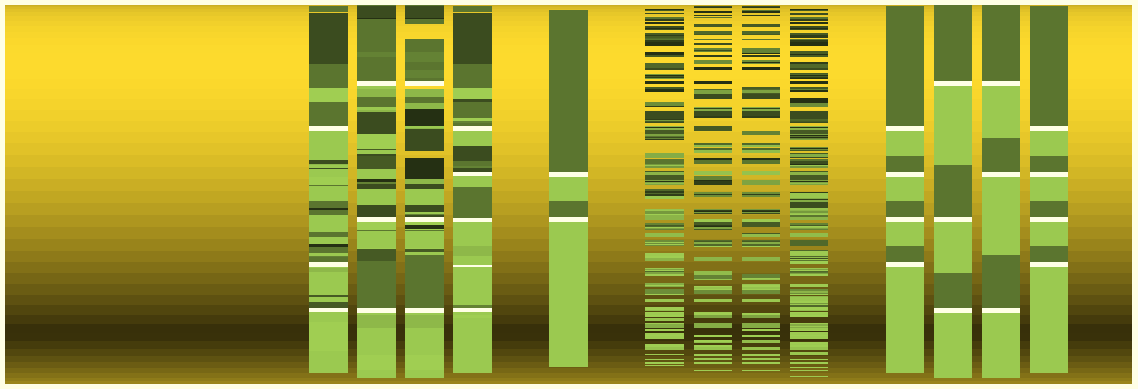
\includegraphics[width=.99\textwidth]{imagenes/minutos-cortos}  
  \caption{Antonia muestra que los haces de los minutos, también,
    deben extenderse un tanto en el tiempo.}
  \label{fig:minutos-cortos}
\end{figure}


---Nooo... ---gimió Cecilia. Y tras unos instantes,
a\-ña\-\mbox{dió---:} Claro, ahora que los pixeles son menos altos,
los haces de un solo rayo resultan prácticamente `instantáneos'. En
fin, no parece tan difícil de solucionar ---y recuperando el teclado
se dispuso a enmendar ambos problemas con renovado optimismo.

\begin{lstlisting}
module reloj_de_sol_continuo(){
  delta_y=ancho_pixel+delta_ancho;
  difference(){
    cuerpo(largo_reloj);    
    // unidades de minuto
    translate([0,8.5*delta_y,0])
      digito(0,alfa(9),alfa(15+10/60));  
    // decenas de minuto
    translate([0,3.5*delta_y,0]){
      for(hora=[9:14],
          minutos=[0,20,40]){
            minuto_decenas=n_a_digito(minutos,1);
            digito(minuto_decenas,
                   alfa(hora+minutos/60),
                   alfa(hora+(minutos+10)/60));
            }
       digito(0,alfa(15),alfa(15+10/60));
       }            
    // separador
    separador(alfa(9),alfa(15+10/60));  
    // unidades de hora
    translate([0,-3.5*delta_y,0])
      for(hora=[9:15]){
        hora_unidades=n_a_digito(hora,0);
        digito(hora_unidades,
               alfa(hora),
               alfa(hora<15 ? hora+50/60 : hora+10/60));
      }        
  }  
}
$vpr=[90-alfa(12+50/60),0,90];
reloj_de_sol_continuo();
\end{lstlisting}%$


\begin{figure}[ht]
  \centering
  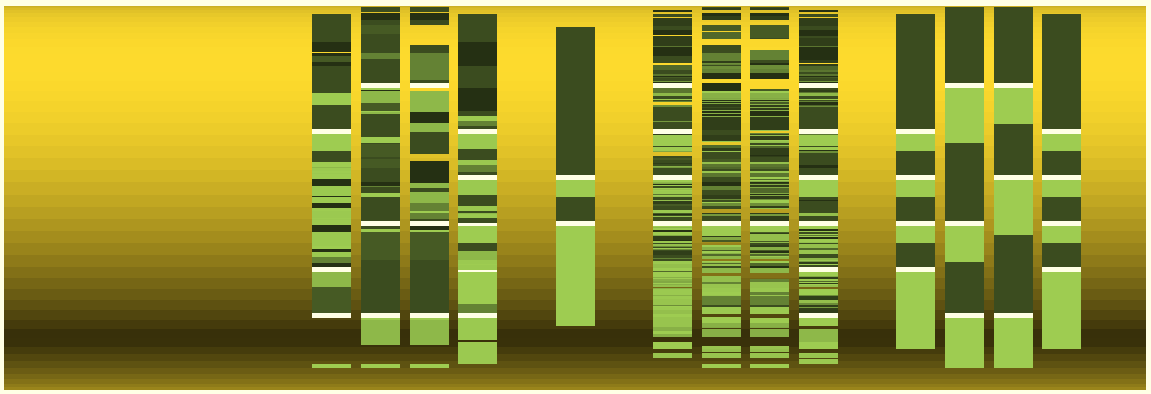
\includegraphics[width=\textwidth]{imagenes/minutos-bien}  
  \caption{Cecilia extiende la duración de los haces de las decenas de
    los minutos.}
  \label{fig:minutos-bien}
\end{figure}


Lo más fácil fue coordinar las horas de todos los elementos: bastó con
modificar las líneas 7 (para las unidades de los minutos), la 10 (para
sus decenas) y la 20 (para el separador).  Quitó también el
\lstinline!if! que precedía a la creación de las decenas de los
minutos (ya que las 6:00 quedaban automáticamente excluidas por la
misma definición del bucle correspondiente), pero agregó en la línea
17 el caso especial del `0' de las 15:00, puesto que resultaba más
difícil incluirlo en dicho bucle.

Por otro lado, para que las decenas de los minutos duraran lo más
posible extendió 10 minutos sus respectivos haces en la línea 15. Lo
que más le costó fue decidirse por ese valor en particular; probó
varios intervalos, aunque ninguno la satisfizo del todo: si el
intervalo era muy breve los dígitos se apagaban muy pronto, y si era
muy grande algunos pixeles se colaban en dígitos vecinos. Esto último,
de todas maneras, ocurría incluso en algunas horas aunque en menor
medida empleando los 10 minutos elegidos: supuso, quizá con más
cansancio que convicción, que con tantos haces de luz atravesando el
reloj tal comportamiento sería inevitable.\footnote{Quedan como
  ejercicios para el lector la busca de otros valores para las
  variables del reloj que eviten ésta y cualquier otra imperfección,
  así como el logro de un mundo perfecto.}

\begin{lstlisting}
$vpr=[90-alfa(12+30/60),0,90];
reloj_de_sol_continuo();
\end{lstlisting}%$


\begin{figure}[ht]
  \centering
  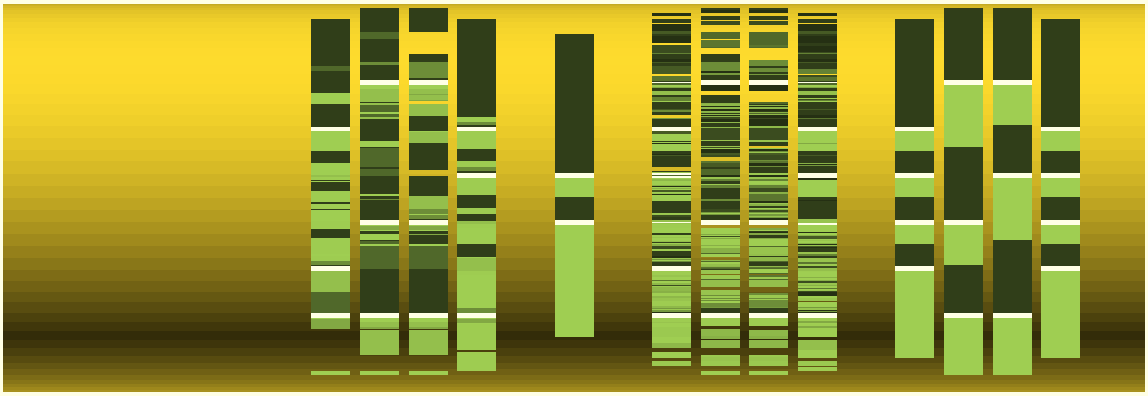
\includegraphics[width=1\textwidth]{imagenes/minutos-imperfectos}  
  \caption{Cecilia comprueba con resignación y melancolía que su
    solución para la duración de las decenas de los minutos no es tan
    ideal como soñaba.}
  \label{fig:minutos-imperfectos}
\end{figure}


---Las 12:20, que deben mostrarse a las 12:30, quedan un poco `sucias'
con pixeles del `4' vecino encendidos ---se lamentó Cecilia en voz
alta, requiriendo así la opinión de su amiga, o tal vez su consejo.

---A mí me pasó lo mismo ---fue la lacónica respuesta de Antonia.

\subsection{Las decenas de la hora}

Lo que restaba parecía tan fácil como las unidades de los minutos: tan
solo un `1' constante.

\begin{lstlisting}
module reloj_de_sol_continuo(){
  delta_y=ancho_pixel+delta_ancho;
  difference(){
    cuerpo(largo_reloj);    
    // unidades de minuto
    translate([0,8.5*delta_y,0])
      digito(0,alfa(9),alfa(15+10/60));  
    // decenas de minuto
    translate([0,3.5*delta_y,0]){
      for(hora=[9:14],
          minutos=[0,20,40]){
            minuto_decenas=n_a_digito(minutos,1);
            digito(minuto_decenas,
                   alfa(hora+minutos/60),
                   alfa(hora+(minutos+10)/60));
            }
       digito(0,alfa(15),alfa(15+10/60));
       }            
    // separador
    separador(alfa(9),alfa(15+10/60));  
    // unidades de hora
    translate([0,-3.5*delta_y,0])
      for(hora=[9:15]){
        hora_unidades=n_a_digito(hora,0);
        digito(hora_unidades,
               alfa(hora),
               alfa(hora<15 ? hora+50/60 : hora+10/60));
      }        
    // decenas de hora
    translate([0,-8.5*delta_y,0])
      digito(1,alfa(10),alfa(15+10/60));    
  }  
}  
$vpr=[90-alfa(12+40/60),0,90];
reloj_de_sol_continuo();
\end{lstlisting}%$

Cecilia casi no se sorprendió al comprobar que bastaban sólo dos
líneas: la 30 ---que ubicaba el `1' en su debido lu\-gar--- y la 31
---que lo desplegaba desde las 10 hasta las 15:10.


\begin{figure}[ht]
  \centering
  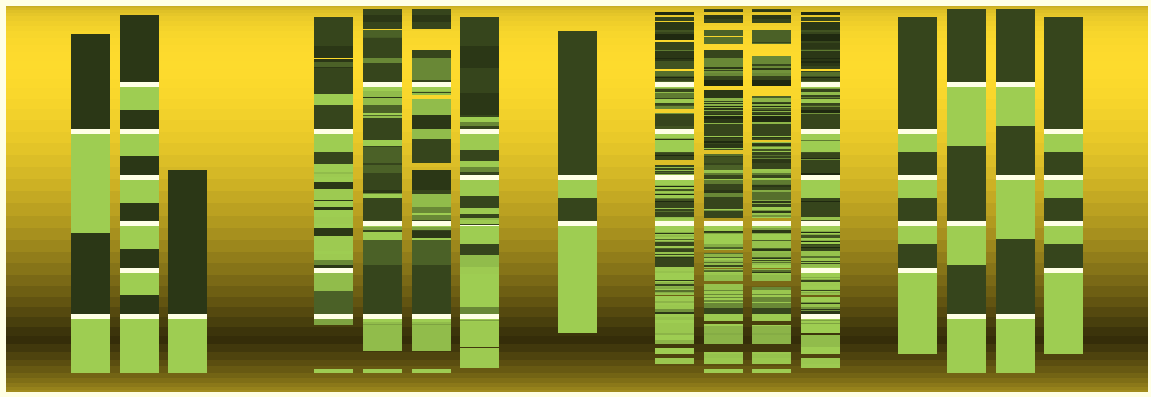
\includegraphics[width=\textwidth]{imagenes/horas-decenas-1}  
  \caption{Cecilia horada el reloj con el \texttt{1} de las decenas de las
    horas.}
  \label{fig:horas-decenas-1}
\end{figure}


Cecilia se recostó blandamente contra el respaldo de la silla; dirigía
su mirada alternativamente al monitor y a Antonia. Quizás esperaba de
ella alguna objeción, u observación que implicara una nueva dilación
en la conquista del reloj. Pero su amiga sólo le devolvía la mirada,
sonriendo.

---¿Y? ---se animó por fin a preguntar---. ¿Ya está?

---Yo diría que sí. Ya está ---respondió Antonia.

---Así que ya está ---fue lo único que Cecilia pudo deslizar, en un
susurro.

Ya estaba.

%\iftoggle{libro}{}{\clearpage} %% comentar para ebook

%\vfill

\begin{figure}[ht]
  \centering
  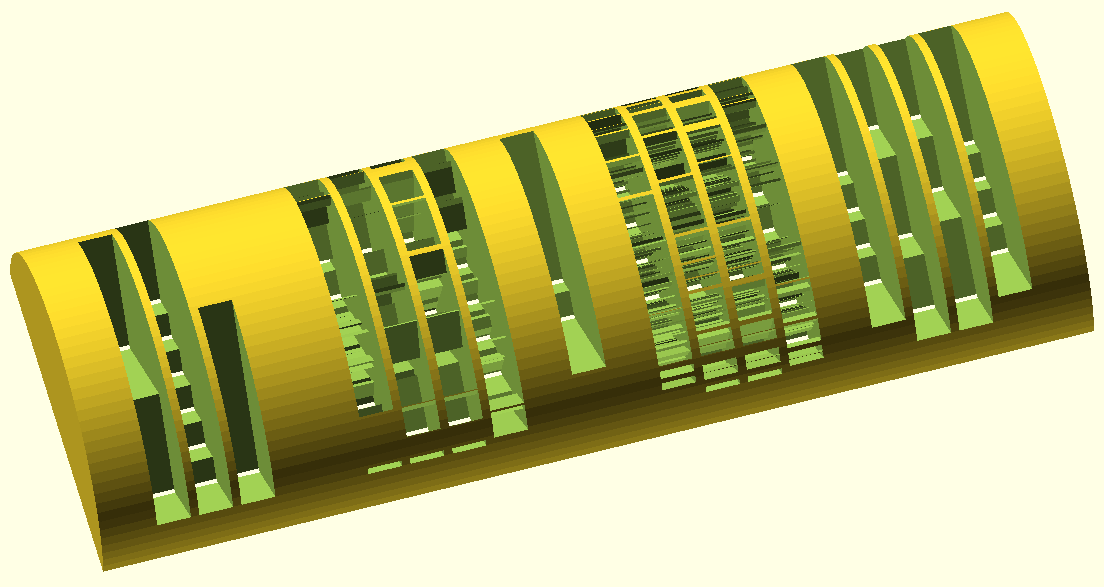
\includegraphics[width=1\textwidth]{imagenes/horas-decenas-2}  
  \caption{Cecilia y Antonia logran finalmente su reloj de Sol
    digital.}
  \label{fig:horas-decenas-2}
\end{figure}

%\vfill


%%% Local Variables:
%%% mode: latex
%%% TeX-master: "../libro"
%%% End:
